\newpage
\section{The Nature of Software}
\subsection{Defining Software}
Software is: 
\begin{enumerate}
    \item instructions (computer programs) that when executed provide desired features, function, and performance; 
    \item data structures that enable the programs to adequately manipulate information; 
    \item documents that describes the operation and use of the programs.
\end{enumerate}

Science 是解释,  Engineering 是创造.

\subsubsection{The Difficulties of Engineering Software}
软件不会磨损, 但环境改变, 其需求也要改变.

软件的本质是要支持需求的改变.

\subsection{Defining the Discipline}
The application of a systematic, disciplined, quantifiable approach
to the development, operation, and maintenance of software; that is, the application of engineering to software.


\begin{figure}[!htb]
    \centering
    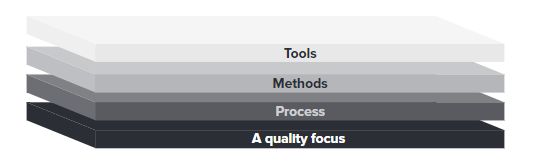
\includegraphics[width=0.42\textwidth]{pic/SE1/A layered technology}
    \caption{A layered technology}
\end{figure}


\subsection{The Software Process}
\subsubsection{The Process Framework}
\begin{enumerate}
    \item Communication(需求分析)
    \item Planning(总体设计)
    \item Modeling(详细设计)
    \item Construction(编码与测试)
    \item Deployment(维护, 版本升级)
\end{enumerate}

\subsubsection{Umbrella Activities}
随便看看

\subsection{Software Engineering Practice}
\subsubsection{General Principles}
\begin{itemize}
    \item KISS (Keep It Simple, Stupid!)
    \item Plan Ahead for Reuse
\end{itemize}

